\chapter{Introduction}

%-------------------------------------------------------------------------------------------------------

\section{Background}

\noindent
Provide a context to the reader, talk about the project, where the idea came from (extension of 3rd Project), some examples of courier robots today. Summary of the big industry players like Google and Amazon. Why is the project unique. Most of this can be taken from the background provided with the project proposal and literature review submissions for Research Skills.\\

\noindent
The ability to select a path to a destination, negotiate obstacles, and anticipate the movement of other people is something that you probably take for granted. To a human these skills are a part of everyday life and do not at first appear to be particularly special, until you try to replicate them. Programming a machine to deal with rush hour traffic or road closures is surprisingly difficult but that has not stop us from trying \cite{MIT}.\\

\newpage

%-------------------------------------------------------------------------------------------------------

\section{Motivation}

\noindent
The motivation for this project was driven by the shortcomings of the last project \cite{JMD14} that we were involved in. In \cite{JMD14} the objective had been to build a fully autonomous robot capable of actively mapping and navigating its environment. Unfortunately this goal proved unrealistic given the time and resources available to the team, and due to the high learning curve and low-end hardware only the mapping functionality was implemented. Essentially this project is being driven by the failure of its predecessor, however this time it is not limited to just the implementation but also the analysis of robotic path planners and their effectiveness. \\

\noindent
Another issue that we noticed during our initial research into path planners for robotic systems was the amount of choice when it came to algorithms. Each planner claimed to be that little be better than another by being faster at planning or producing shorter paths. Selecting the ``best'' planner can be incredibly difficult for a newcomer as up until now there has been no detailed comparison of these planners. Documenting how some of the most popular planners perform against each other will not only provide us with a valuable insight but also countless other newcomers to robotic navigation. 

\newpage

%-------------------------------------------------------------------------------------------------------

\section{Scope Definition}

\noindent
What is the actual scope of this project? Defining what to exclude is just as important as what is included so state both of these here in bullet points:\\

\noindent
The scope of this project \textbf{includes}:
\begin{itemize}
\item Path Planning: calculating the shortest and safest path to the delivery point.

\item State everything else...
\end{itemize}

\noindent
The following are \textbf{outside} the scope of this project:
\begin{itemize}
\item Collection: purely automated collection using beacons or computer vision. Goods will be manually handled by a human operator.

\item State everything else...
\end{itemize}

\newpage

%-------------------------------------------------------------------------------------------------------

\section{Research Question(s)}

\noindent
Primary research question

\noindent
The project will aim to address the following additional research questions:

\begin{itemize}
\item What advances to date have been made in navigation systems for mobile robots?

\item How important is navigation with respect to robotics?

\item Will it be possible to develop a generic navigation system that is independent from the hardware architecture for delivery robots?

\end{itemize}

%-------------------------------------------------------------------------------------------------------

\section{Objectives}

\noindent
This project has a set number of objectives which are:

\begin{itemize}
\item To produce a literature review covering the advancements in autonomous navigation in robotic systems.

\item To develop and test a generic hardware independent navigation system for ground based mobile robots. 

\item To evaluate the effectiveness of path planning techniques in known environments. 

\item To assess the benefits of faster planning times against path traversal lengths.

\item To test the solution against a set of predefined challenges and evaluate its performance.

\end{itemize}

\newpage

%-------------------------------------------------------------------------------------------------------

\section{Feasibility}
\noindent
This project is being supervised by Prof. Arnold Hensman who has spent at least 3 years working in the research area and has supervised past projects in robotics including one that the candidate participated in \cite{JMD14}. It will build upon the work of a past project \cite{JMD14} whichs support the hypothesis that autonomous navigation can be implemented with similar resources. The project has well defined requirements, milestones, deliverables, and the purposed candidate has already spent over a year working in the research area. \newline

\noindent
Most of the technical resources required to achieve this project's goals are already available, including a code base, all other required equipment such as a high quality laser range finder are on order. Two separate robotic systems with the core functionality needed to implement the purposed system already exist and are ready for development (Figure: \ref{Figure: Robot Platforms.}). 
\newline

\begin{figure}[htbp]

\center 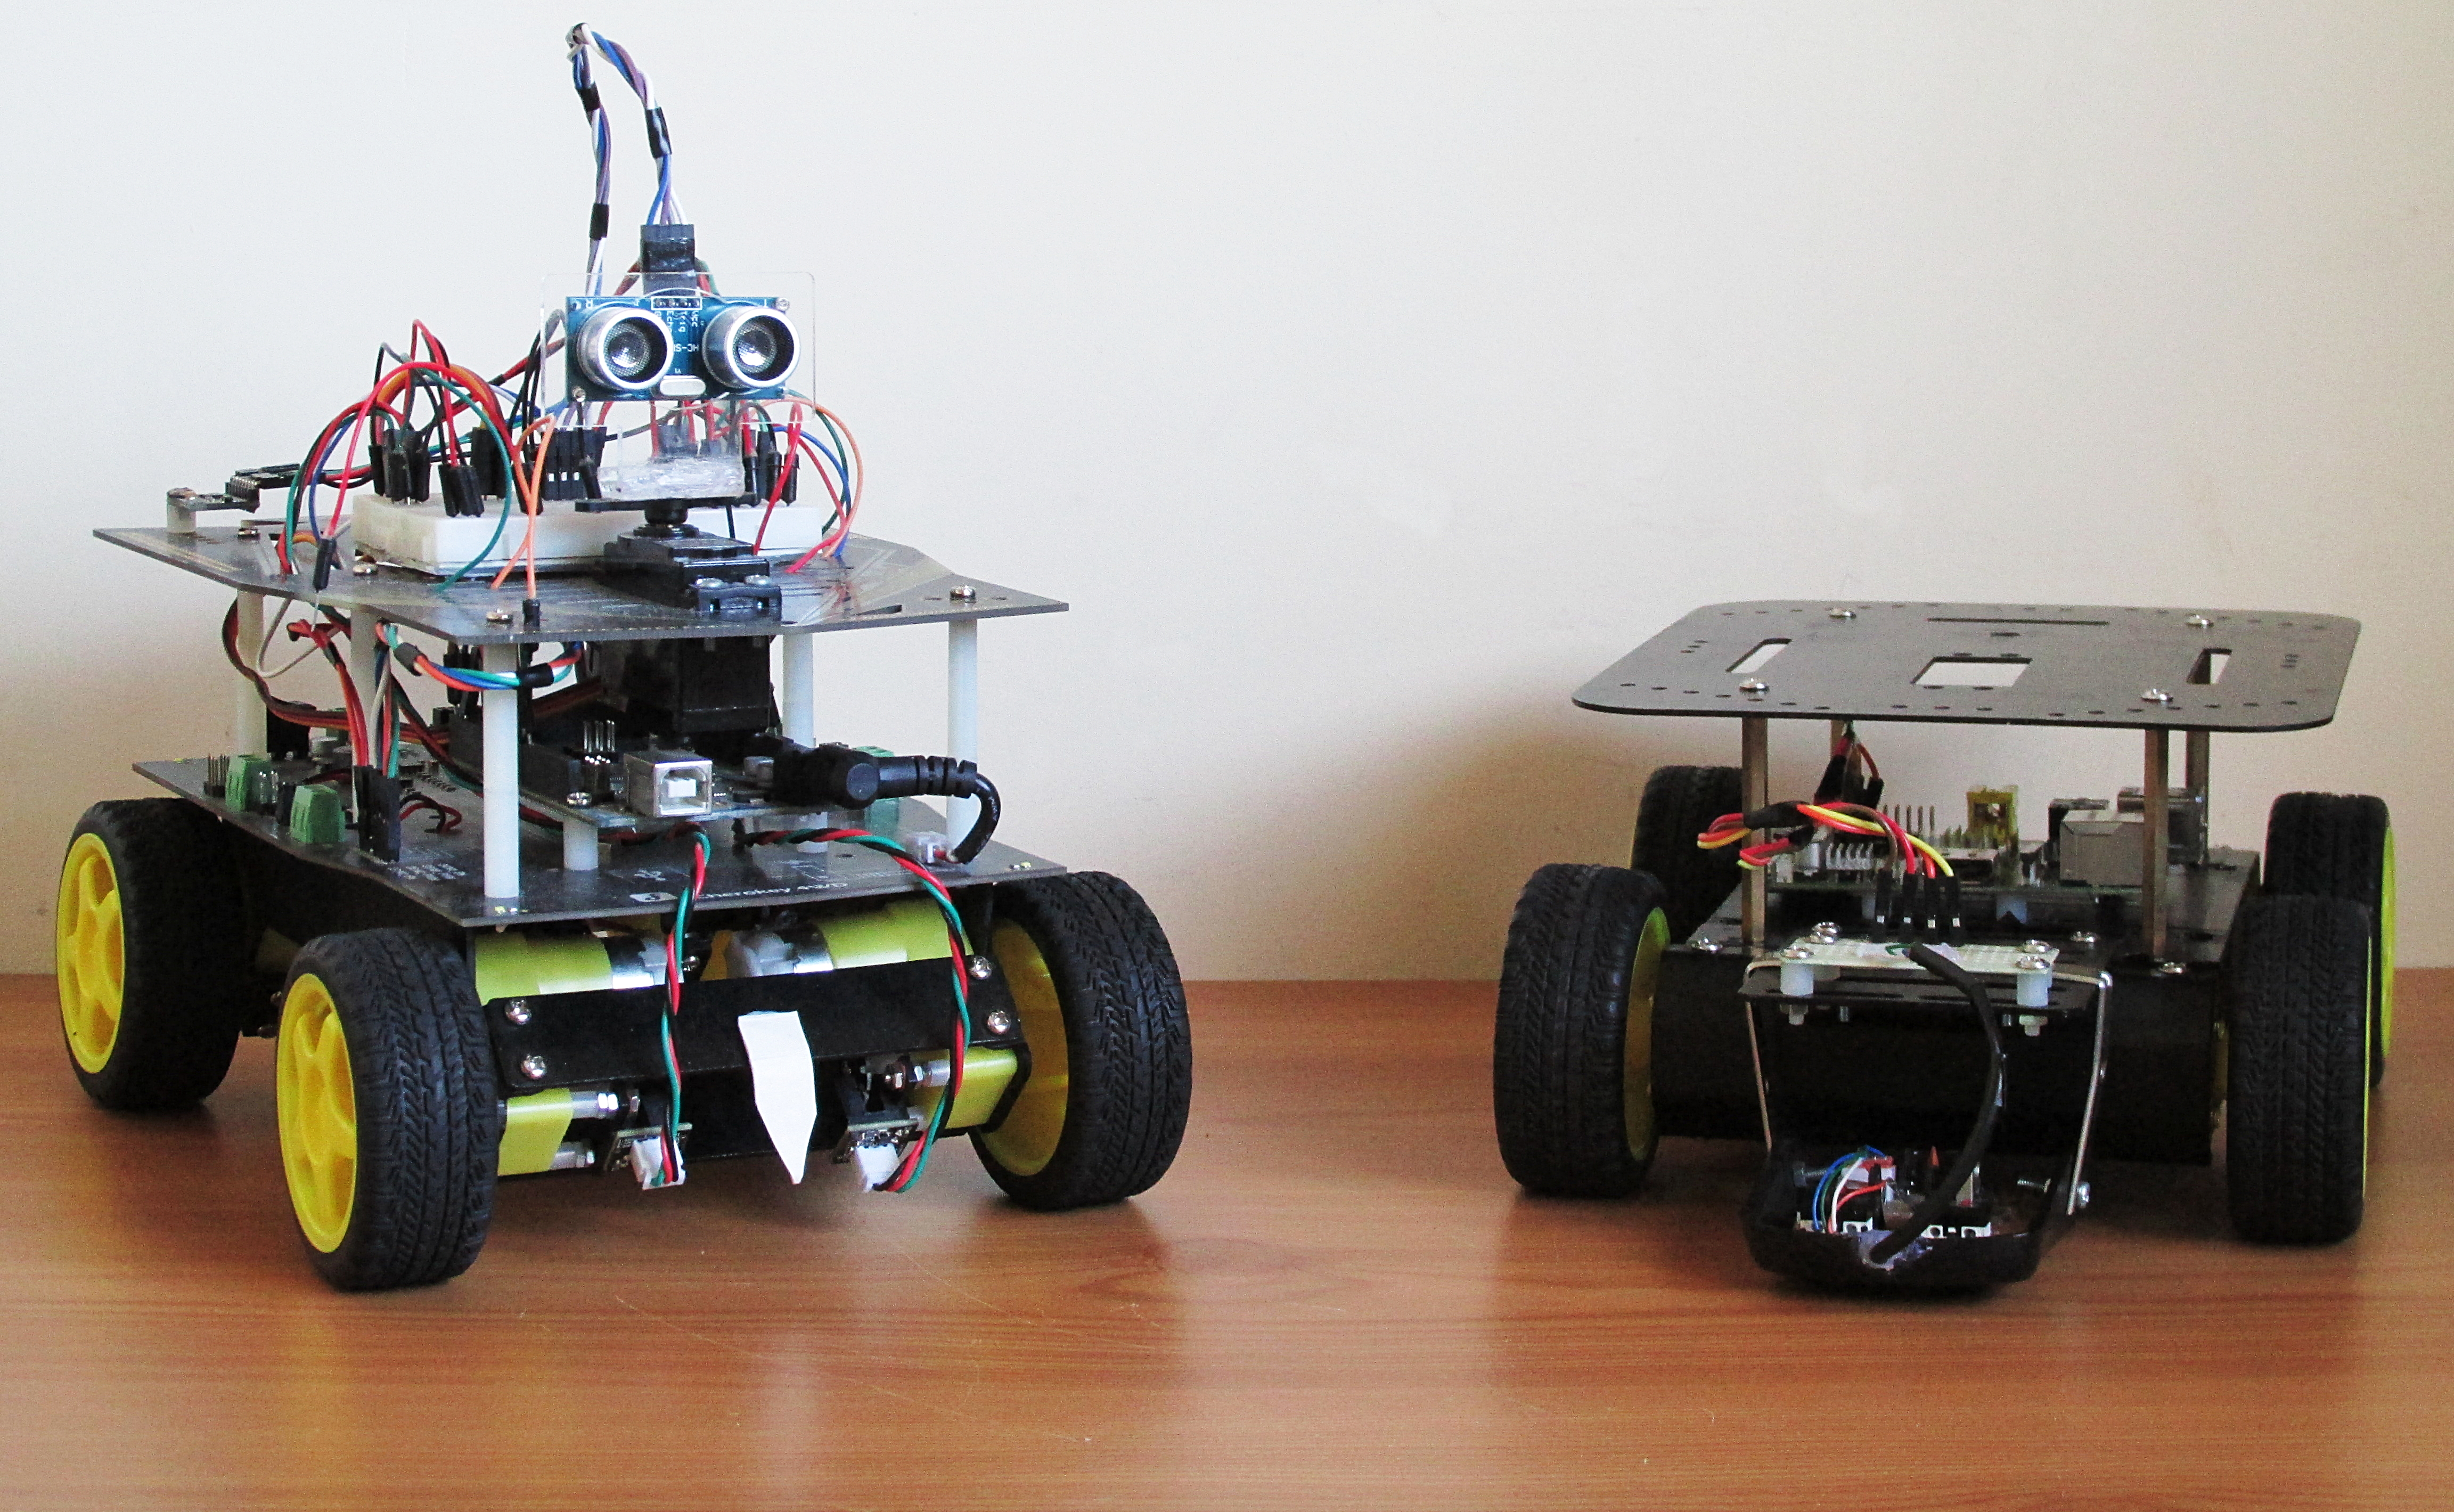
\includegraphics[width=230pt]{illustrations/robots}\\
\caption{The candidate's Cherokey robot and ITB's Pirate platform.} 
\label{Figure: Robot Platforms.}

\end{figure}
